\documentclass{beamer}
\usepackage[utf8]{inputenc}

\usetheme{Madrid}
\usecolortheme{default}
\usepackage{amsmath}
\usepackage{amssymb,amsfonts,amsthm}
\usepackage{txfonts}
\usepackage{tkz-euclide}
\usepackage{listings}
\usepackage{adjustbox}
\usepackage{array}
\usepackage{tabularx}
\usepackage{gvv}
\usepackage{lmodern}
\usepackage{circuitikz}
\usepackage{tikz}
\usepackage{graphicx}

\setbeamertemplate{page number in head/foot}[totalframenumber]

\usepackage{tcolorbox}
\tcbuselibrary{minted,breakable,xparse,skins}



\definecolor{bg}{gray}{0.95}
\DeclareTCBListing{mintedbox}{O{}m!O{}}{%
  breakable=true,
  listing engine=minted,
  listing only,
  minted language=#2,
  minted style=default,
  minted options={%
    linenos,
    gobble=0,
    breaklines=true,
    breakafter=,,
    fontsize=\small,
    numbersep=8pt,
    #1},
  boxsep=0pt,
  left skip=0pt,
  right skip=0pt,
  left=25pt,
  right=0pt,
  top=3pt,
  bottom=3pt,
  arc=5pt,
  leftrule=0pt,
  rightrule=0pt,
  bottomrule=2pt,
  toprule=2pt,
  colback=bg,
  colframe=orange!70,
  enhanced,
  overlay={%
    \begin{tcbclipinterior}
    \fill[orange!20!white] (frame.south west) rectangle ([xshift=20pt]frame.north west);
    \end{tcbclipinterior}},
  #3,
}
\lstset{
    language=C,
    basicstyle=\ttfamily\small,
    keywordstyle=\color{blue},
    stringstyle=\color{orange},
    commentstyle=\color{green!60!black},
    numbers=left,
    numberstyle=\tiny\color{gray},
    breaklines=true,
    showstringspaces=false,
}
\title{1.2.25}
\date{25th March, 2026}
\author{Vishwambhar - EE25BTECH11025}

\begin{document}

\frame{\titlepage}
\begin{frame}{Question}
Let $x\brak{t}$ be a continuous-time, real-valued signal band-limited to $F$ Hz. The Nyquist sampling rate, in Hz, for $y\brak{t}=x\brak{0.5t}+x\brak{t}-x\brak{2t}$ is
\begin{enumerate}
    \item $F$
    \item $2F$
    \item $4F$
    \item $8F$
\end{enumerate}
\end{frame}

\begin{frame}{Definition of Nyquist Rate}
Given Bandwidth of the signal is $F$.\\
Nyquist rate = 2 × highest frequency component of the signal.\\
Fourier transform of a scaled signal will be:
\begin{align}
x(at)\xleftarrow{}\mathcal{F}\xrightarrow{} \frac{1}{|a|} \, X\brak{\frac{f}{a}}\\
X\brak{f}=0 \quad\text{for} |f|>F
\end{align}
\end{frame}

\begin{frame}{Bandwidth of scaled signals}
For $x\brak{0.5t}$\\
Here a= 0.5, from eq. $\brak{1}$
\begin{align}
    x(0.5t)\xleftarrow{}\mathcal{F}\xrightarrow{} \frac{1}{|0.5|} \\
    \text{from eq (2)}\\
    |2f|\leq F\Rightarrow|f|\leq \frac{F}{2}
\end{align}
Bandwidth = $0.5F$
\end{frame}

\begin{frame}{Bandwidth of scaled signals}
For $x\brak{2t}$\\
Here a= 2, from eq. $\brak{1}$
\begin{align}
    x(2t)\xleftarrow{}\mathcal{F}\xrightarrow{} \frac{1}{|2|} \\
    \text{from eq (2)}\\
    |0.5f|\leq F\Rightarrow|f|\leq 2F
\end{align}
Bandwidth = $2F$
For $x(t)$ bandwidth will be same.
\end{frame}


\begin{frame}{Bandwidth of combined signal}
It will be the maximum of the of all bandwidths.
\begin{align}
B=2F
\end{align}
\end{frame}

\begin{frame}{Nyquist Rate}
Finding Nyquist rate from definition.
\begin{align}
2\times B = 2\times 2F=4F
\end{align}
\end{frame}

\begin{frame}{Plot-x(t)}
    \begin{figure}
        \centering
        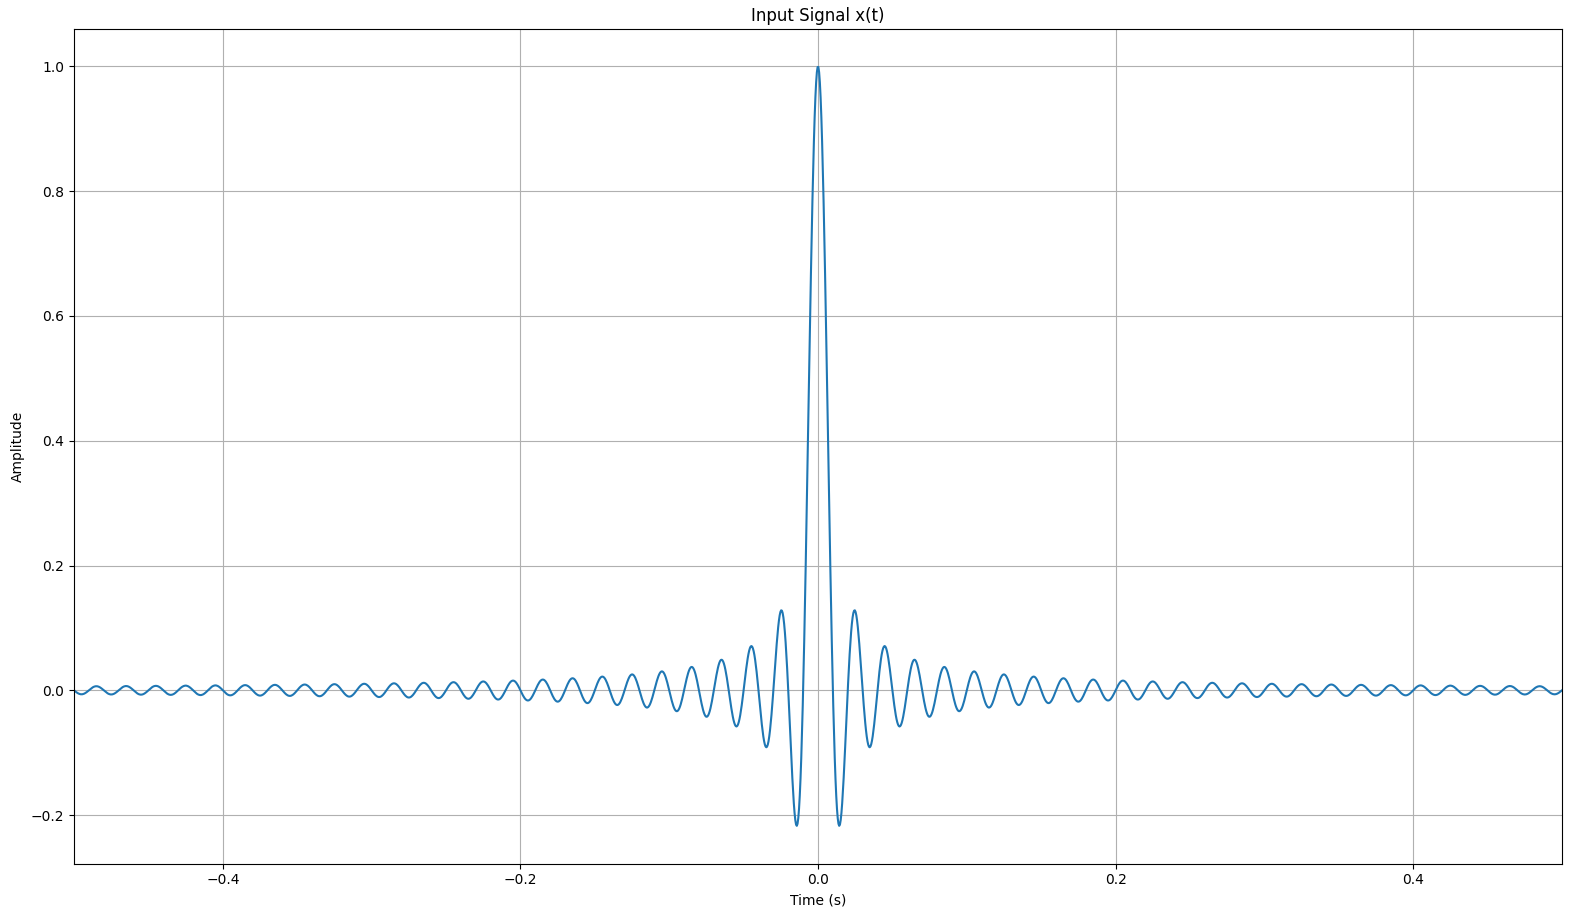
\includegraphics[width=1\columnwidth]{figs/xoft.png}
        \label{fig:fig}
    \end{figure}
\end{frame}

\begin{frame}{Plot-y(t)}
    \begin{figure}
        \centering
        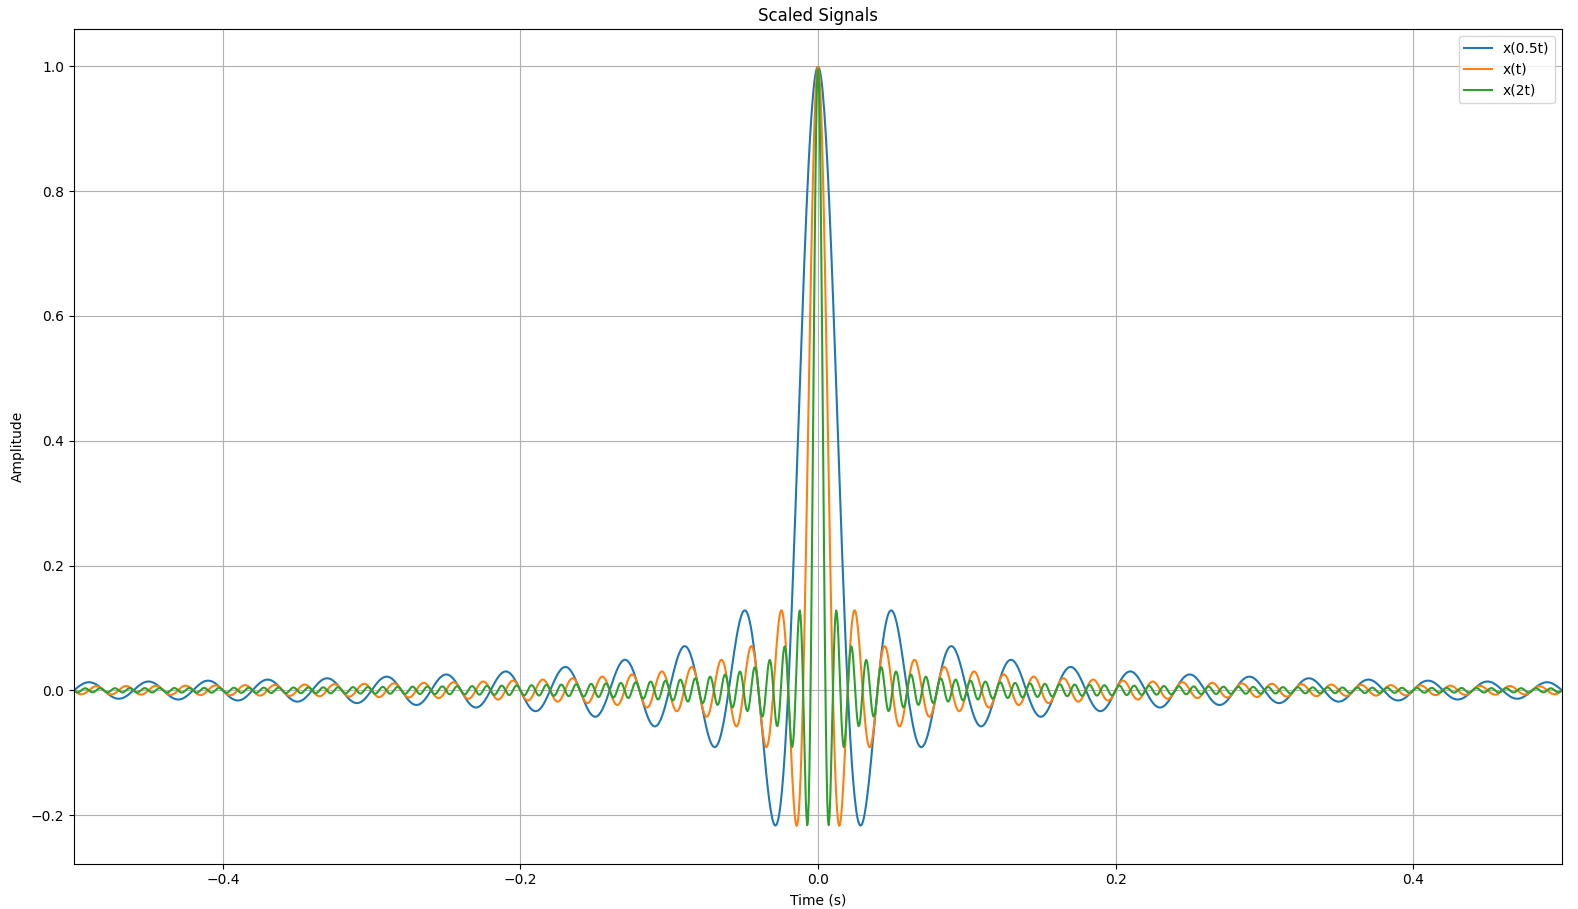
\includegraphics[width=1\columnwidth]{figs/alloft.png}
        \label{fig:fig}
    \end{figure}
\end{frame}

\begin{frame}{Plot-y(t)}
    \begin{figure}
        \centering
        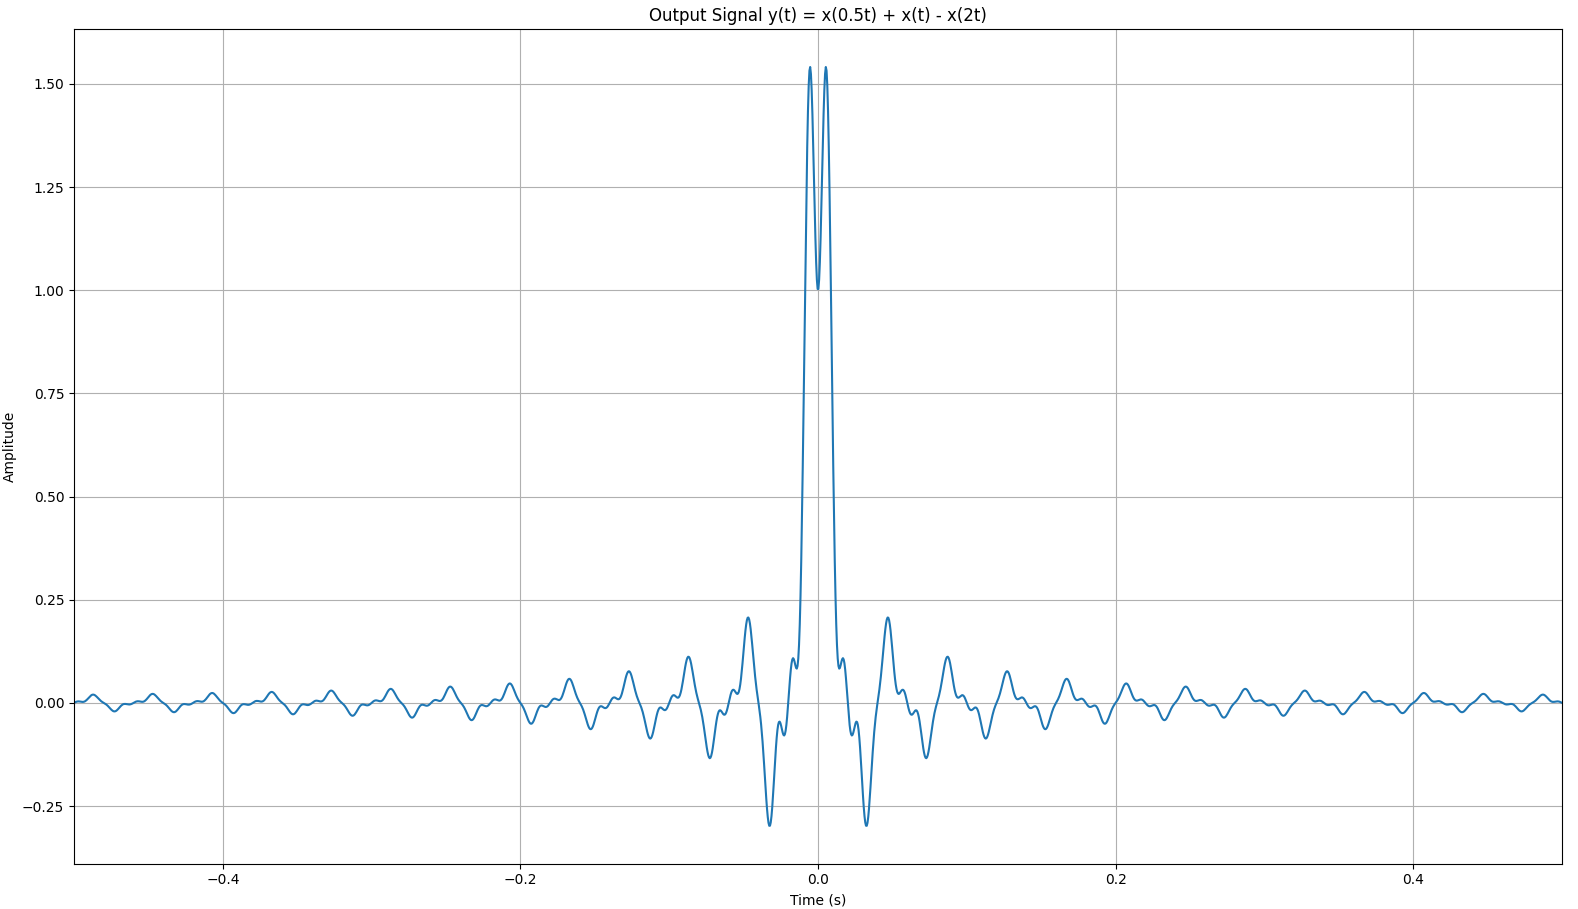
\includegraphics[width=1\columnwidth]{figs/yoft.png}
        \label{fig:fig}
    \end{figure}
\end{frame}

\begin{frame}{Spectrum of x(t)}
    \begin{figure}
        \centering
        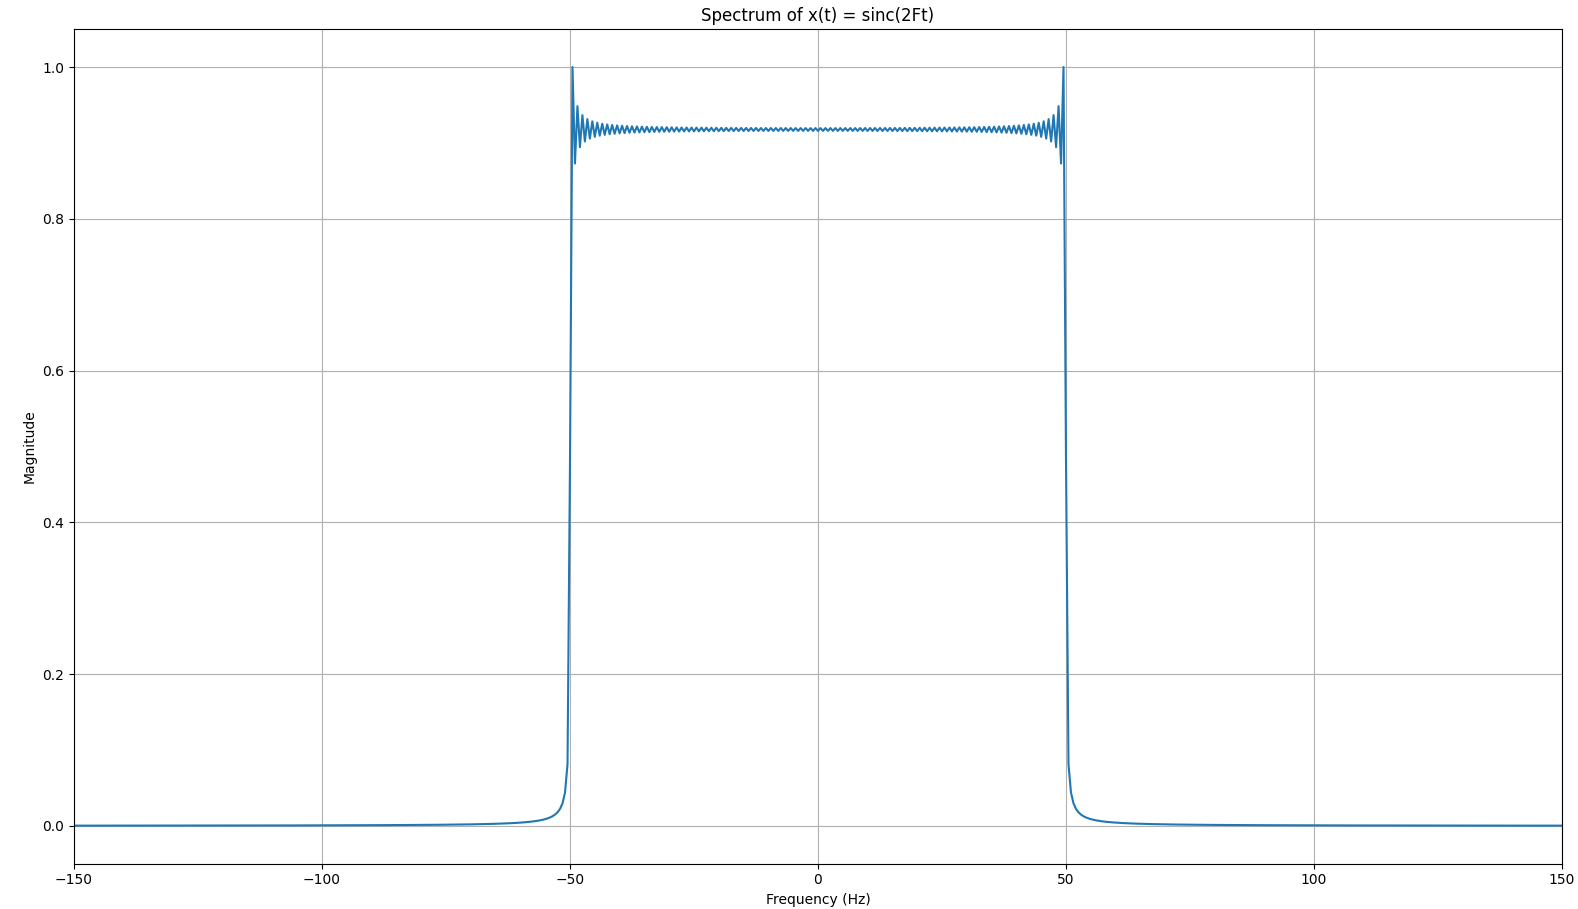
\includegraphics[width=1\columnwidth]{figs/soxt.png}
        \label{fig:fig}
    \end{figure}
\end{frame}

\begin{frame}{Spectrum of y(t)}
    \begin{figure}
        \centering
        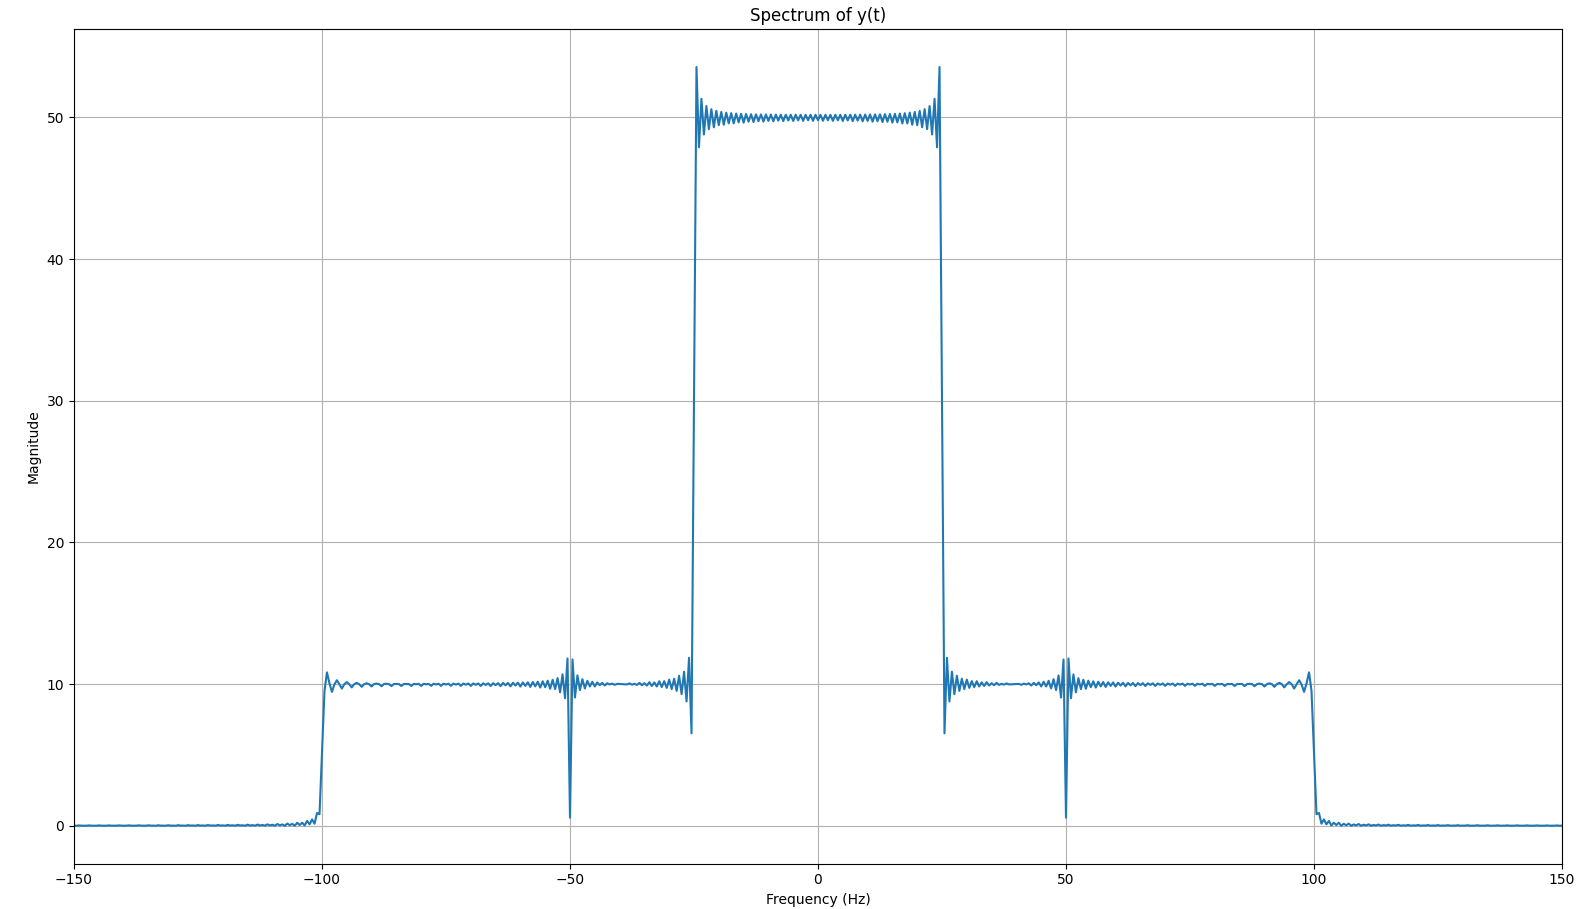
\includegraphics[width=1\columnwidth]{figs/soyt.png}
        \label{fig:fig}
    \end{figure}
\end{frame}

\begin{frame}[fragile]
    \frametitle{Python Code 1}
    \begin{lstlisting}
import numpy as np
import matplotlib.pyplot as plt
Fs = 2000
T = 2
t = np.linspace(-T/2, T/2, Fs*T)
F = 50
x = np.sinc(2 * F * t)

def scale_signal(x, t, scale):
    t_scaled = t * scale
    return np.interp(t_scaled, t, x, left=0, right=0)

x_05 = scale_signal(x, t, 0.5)
x_1  = x
x_2  = scale_signal(x, t, 2)
y = x_05 + x_1 - x_2
    \end{lstlisting}
\end{frame}

\begin{frame}[fragile]
    \frametitle{Python Code 1}
    \begin{lstlisting}

def compute_fft(signal, Fs):
    N = len(signal)
    X = np.fft.fftshift(np.fft.fft(signal))
    f = np.fft.fftshift(np.fft.fftfreq(N, d=1/Fs))
    return f, np.abs(X)

f_x, X = compute_fft(x, Fs)
X = X / np.max(X)

plt.figure()
plt.plot(f_x, X)
plt.title("Spectrum of x(t) = sinc(2Ft)")
plt.xlabel("Frequency (Hz)")
plt.ylabel("Magnitude")

plt.xlim(-150, 150)
plt.grid()
plt.show()
    \end{lstlisting}
\end{frame}

\begin{frame}[fragile]
    \frametitle{Python Code}
    \begin{lstlisting}
f, Y = compute_fft(y, Fs)

def estimate_bandwidth(f, spectrum, threshold=0.05):
    spectrum = spectrum / np.max(spectrum)
    indices = np.where(spectrum > threshold)[0]
    if len(indices) == 0:
        return 0
    max_freq = np.max(np.abs(f[indices]))
    return max_freq
bandwidth = estimate_bandwidth(f, Y)
nyquist_rate = 2 * bandwidth
print("Estimated Bandwidth:", bandwidth, "Hz")
print("Estimated Nyquist Rate:", nyquist_rate, "Hz")
plt.figure()
plt.plot(f, Y)
plt.title("Spectrum of y(t)")
plt.xlabel("Frequency (Hz)")
plt.ylabel("Magnitude")
plt.xlim(-150, 150)
plt.grid()
plt.show()
    \end{lstlisting}
\end{frame}

\begin{frame}[fragile]
    \frametitle{Python Code 2}
    \begin{lstlisting}
import numpy as np
import matplotlib.pyplot as plt

Fs = 2000
T = 2
t = np.linspace(-T/2, T/2, Fs*T)
F = 50
x = np.sinc(2 * F * t)

def scale_signal(x, t, scale):
    t_scaled = t * scale
    return np.interp(t_scaled, t, x, left=0, right=0)

x_05 = scale_signal(x, t, 0.5)
x_1  = x
x_2  = scale_signal(x, t, 2)
y = x_05 + x_1 - x_2
    \end{lstlisting}
\end{frame}

\begin{frame}[fragile]
    \frametitle{Python Code 2}
    \begin{lstlisting}
plt.figure()
plt.plot(t, x)
plt.title("Input Signal x(t)")
plt.xlabel("Time (s)")
plt.ylabel("Amplitude")
plt.xlim(-0.5, 0.5)
plt.grid()
plt.show()

plt.figure()
plt.plot(t, x_05, label="x(0.5t)")
plt.plot(t, x_1, label="x(t)")
plt.plot(t, x_2, label="x(2t)")
plt.title("Scaled Signals")
    \end{lstlisting}
\end{frame}

\begin{frame}[fragile]
    \frametitle{Python Code 2}
    \begin{lstlisting}
plt.title("Scaled Signals")
plt.xlabel("Time (s)")
plt.ylabel("Amplitude")
plt.legend()
plt.xlim(-0.5, 0.5)
plt.grid()
plt.show()

plt.figure()
plt.plot(t, y)
plt.title("Output Signal y(t) = x(0.5t) + x(t) - x(2t)")
plt.xlabel("Time (s)")
plt.ylabel("Amplitude")
plt.xlim(-0.5, 0.5)
plt.grid()
plt.show()
    \end{lstlisting}
\end{frame}
\end{document}
